\chapter[Analiza zmogljivosti obla"cne storitve c9]{Analiza zmogljivosti obla"cne storitve Cloud9}

\pagestyle{fancy}
\fancyhf{}
\fancyhead[LE,RO]{\thepage}
\fancyhead[RE,LO]{\leftmark}

\huge "Ziga Kokelj, Tadej Hiti,\\Miha Bizjak, Matej Kristan
\normalsize
\bigskip

\section{Opis problema}

\noindent Dana"snje dni se uveljavljajo obla"cne storitve, saj so s stali"s"ca uporabnika najenostavnej"se za uporabo. Na"sa naloga je implementirati prenos datoteke na oz. z obla"cne storitve in breme na obla"cni storitvi, za katerega smo si izbrali sortiranje numeri"cnih podatkov.
\noindent Na sliki \ref{8_opis_problema} je grafi"cen prikaz opisanega problema.

\begin{figure}
  \centering
    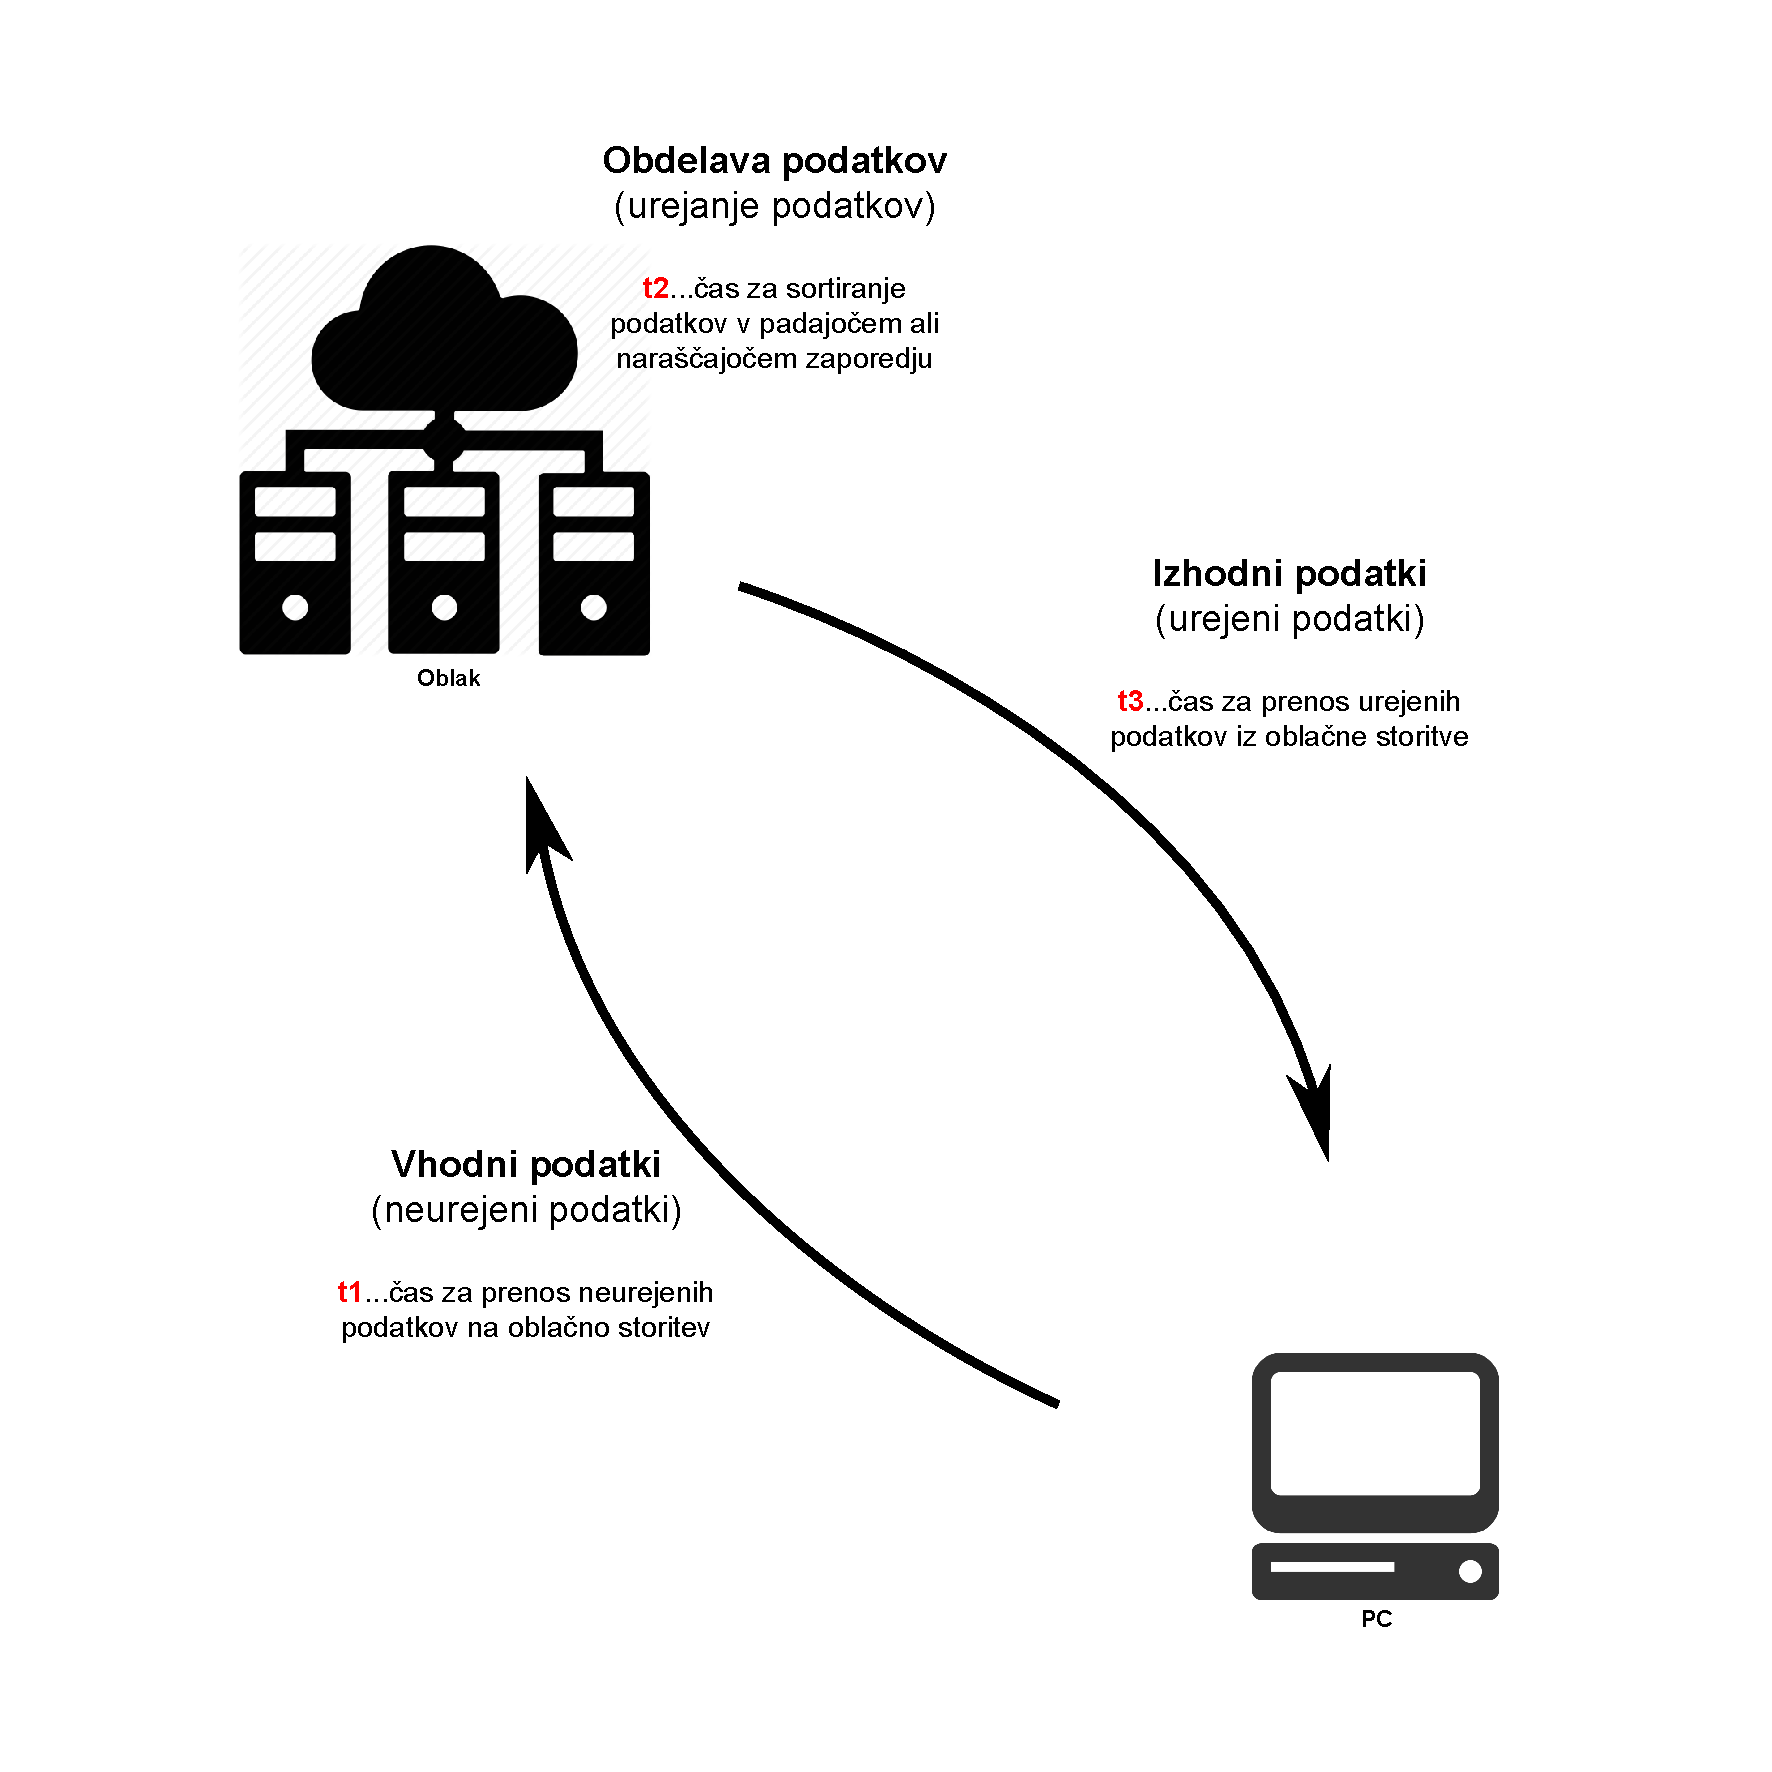
\includegraphics[width=0.8\textwidth]{8_zzrs_opis_problema.pdf}
  \caption{Shema delovanja sistema.}
  \label{8_opis_problema}
\end{figure}


\section{Namen}

Na"se testiranje bo obsegalo merjenje razli"cnih izvajalnih "casov na podlagi katerih bi pri"sli do podatkov o zmogljivosti sistema. Breme sistema bodo razli"cni algoritmi sortiranja podatkov. Namen na"se naloge bo ugotoviti zmogljivost zastonjske ponudbe z vidika razli"cnih metrik zmogljivosti.


\section{Izbira ponudnikov}
Zaradij predhodnih izku"senj z obla"cno storitvijo Cloud9 smo se odlo"cili za njihovo zastonjsko ponudbo. Cloud9 ponuja razvojno okolje in operacijski sistem Ubuntu v katerem lahko pi"semo ali pa izvajamo razli"cne programe.

\subsection{Cloud 9}
Cloud9 je delavno orodje, ki je namenjeno programiranju v brskalniku. Torej vpi"semo URL v brskalnik in "ze imamo vse pripravljeno za pisanje prvega programa. Pri zastonski narocnini nam dajo 512MB pomnilnika.

\section{Izbira tehnologij}
V obla"cni storitvi smo implementirali stre"znik, ki je napisan v jeziku javascript z uporabo knji"znice Node.js~\cite{8_nodejs}, ki v odvisnosti od URL zahteve posreduje temu primerno datoteko na odjemalca. Stre"znik poskrbi za prena"sanje datotek in zagon potrebnega programa za sortiranje podatkov na stre"zniku.

Zaradi avtomatskega testiranja smo napisali tudi skripto v programskem jeziku python~\cite{8_python}, ki omogo"ca avtomatsko po"siljanje datoteke in URL zahteve na stre"znik, ter kot odgovor prejme urejeno datoteko z urejenimi podatki. Seveda pa ob tem "se zabele"zimo "cas pred po"siljanjem zahteve in "cas po prejetju urejene datoteke, da dobimo izvajalni "cas celotne procedure.
